%%%%%%%%%%%%%%%%%%%%%%%%%%%%%%%%%%%%%%%%%%%%%%%%%%%%%%%%%%%%%%%%%%%%%%%%%%%%%%%%%%%%%%%%%%%%%%%%%%%%%%%%%%%%%%%%%%%%%%%%%%%%%%%%%%%%%%%%%%%%%%%%%%%%%%%%%%%%%%%%%%%%%%%%%%%%%%%%%%%%
%%%%%%%%%%%%%%%%%%%%%%%%%%%%%%%%%%%%%%%%%%%%%%%%%%%%%%%%%%%%%%%%%%%%%%%%%%%%%%%%%%%%%%%%%%%%%%%%%%%%%%%%%%%%%%%%%%%%%%%%%%%%%%%%%%%%%%%%%%%%%%%%%%%%%%%%%%%%%%%%%%%%%%%%%%%%%%%%%%%%
\section{Simulated samples}
\label{sec:SimulatedSamples}

For the investigation of the various backgrounds to this search, the analysis relies also on simulated sample.
An extensive introduction to the techniques and tools required for the simulation of SM and beyond SM processes can be found in Section~\ref{FIXME}.

In the following two sections an overview about the used SM (Section~\ref{sec:SMSamples}) and SUSY samples (Section~\ref{sec:SignalSamples}) is given.
All samples are reweighted to match the measured distribution of primary vertices in data.

\subsection{SM Background samples}
\label{sec:SMSamples}
To investigate the sources of background, various simulated SM samples were used.
In order to have the possibility to make use of the $dE/dx$ variables, a special data format of the simulated samples is required (called RECO format).
Unfortunately, not all SM processes were available in this format in which also the information about the energy release in the tracking system is included.
However, as this analysis needs to rely anyways on a data-based background estimation method, because of the limited quality of the $dE/dx$ simulation.
this does not constitute a serious problem, but only limit the possibility of an extensive comparison between data and simulation going beyond shape comparisons.

In Table \ref{tab:SMsamples_RECO} all SM samples are listed which were available in the RECO format and are used in the analysis.
\renewcommand{\arraystretch}{1.5}
\begin{table}[!b]
\centering
\caption{Available and used Standard Model background samples containing $\Delta E/\Delta x$ information.}
\label{tab:SMsamples_RECO}
\makebox[0.99\textwidth]{
\begin{tabular}{lll}
\multicolumn{3}{c}{} \\
\toprule
 Process & Cross section $\left[\pb\right]$ & $\mathcal{O}_{\text{calculation}}$ \\%& Size $\left[\text{TB}\right]$\\
\midrule
 $W$ + jets                                             &  36703.2     &  NNLO \cite{bib:FEWZ} \\%& 70.4 \\
 $t\bar{t}$ + jets                                      &  245.8       &  NNLO \cite{bib:ttbar:Czakon_2013}\\%& 55.9 \\
 Z$\rightarrow\ell\ell$ ($\ell=e,\mu,\tau$)             &  3531.9      &  NNLO \cite{bib:FEWZ} \\%& 5.1  \\
 QCD ($50\gev<\hat{p}_{\text{T}}<1400\gev$)               &  9374794.2    &  LO  \\%% & 44.3\\
\bottomrule
\end{tabular}}
\end{table}  
Due to the immense size of the samples (between 5 and 70\,TB) and in order to match a reasonable storage space a reduction was done by selecting only events which contain at least one leading jet with a minimum transverse momentum of $\pt>60\gev$.

In addition, further simulated samples not containing the energy information are used.
These are needed to study the backgound inclusively in the variable \ias.
They are listed in Table~\ref{tab:SMsamples_AOD}.
\renewcommand{\arraystretch}{1.5}
\begin{table}[!t]
\centering
\caption{Used Standard Model background samples without $\Delta E/\Delta x$ information.}
\label{tab:SMsamples_AOD}
\makebox[0.99\textwidth]{
\begin{tabular}{lll}
\multicolumn{3}{c}{} \\
\toprule
 Process & Cross section $\left[\pb\right]$ & $\mathcal{O}_{\text{calculation}}$ \\%& Size $\left[\text{TB}\right]$\\
\midrule
 $W$ + jets                                                &  36703.2    &  NNLO \cite{bib:FEWZ} \\%& 70.4 \\
 Z$\rightarrow\ell\ell$ ($\ell=e,\mu,\tau$) + 1,2,3,4 jets &  3531.9     &  NNLO \cite{bib:FEWZ} \\%& 5.1  \\
\bottomrule
\end{tabular}}
\end{table}  

%\begin{itemize}
%\item Main Background are ... ???
%\item Most important sample was included: Wjets
%\item ZoNuNu Backgrund not availbale plays also a role (see DT paper!)
%\item Table of SM samples with cross sections
%\end{itemize}

\subsection{Signal samples}
\label{sec:SignalSamples}
For the investigation of a possible signal, events containing either chargino pair production $q\bar{q} \rightarrow \chipm \chimp$ or chargino neutralino production $q\bar{q} \rightarrow \chipm \chiO$ are simulated. 
The simulation is done with the matrix-element event generator \madgraph \cite{bib:Madgraph_2014}
The parton showering and hadronization processes are then simulated with Pythia 6 \cite{bib:Pyhtia6_2006}.
A last step is needed to simulate the interations of the generated particles with the detector material, which is done with \geant \cite{bib:Geant4_2003,bib:Geant4_2006}.

Furthermore, a speacial treatment for long-lived particles is required.
In order to get the right detector simulation of the energy loss of the long-lived particles which decay after the beam pipe, the lifetime of the chargino cannot be set in the matrix-element generator but needs to be specified within \geant.
This also means, that the decay products are only existing in the detector simulation, but are not accessible as particles in the event generators.


To narrow down the required computing sources, the simulation was only done for a few lifetimes (1\cm, 5\cm, 10\cm, 50\cm, 100\cm, 1\,000\cm and 10\,000\cm).
To get still a tight scan over the lifetime space, other lifetimes were generated using lifetime reweighting.
This can be done by determining for every event a weight which is depending on the individual proper lifetime of the chargino (in case of chargino pair production it depends on the individual lifetime of the two charginos).
The event weight is given by
\begin{equation*}
w = \prod_{i=1}^n \frac{\tau^{\text{gen}}}{\tau^{\text{target}}}\cdot  \exp \left[ t_i \cdot \left( \frac{1}{\tau^{\text{target}}} - \frac{1}{\tau^{\text{gen}}} \right) \right] ,
\end{equation*}
where $n$ is the  number of charginos in the event, $\tau^{\text{gen}}$ is the generated mean lifetime in the particle's rest frame and $t_i$ is the individual proper lifetime of the chargino. 
The resulting mean lifetime is then given by $\tau^{\text{target}}$. A derivation of this formula can be found in Appendix~\ref{blabla}.
With the reweighting procedure a tight covering of the lifetime space could be achieved with lifetimes of \ctau = $a\cdot10^{n}$ for $n$=0,1,2,3,4 and $a$=$\left[1,9\right]$.
Figure~\ref{blabla} shows the exponential distribution of the individual proper lifetime of the charginos after reweighting a simulated sample with $c\tau^{\text{gen}}=50\cm$ to a lifetime of $c\tau^{\text{target}}=10\cm$.
Fitting the exponential spectrum should result in the correct mean proper lifetime as parameter of the fit.
It can be seen, that the reweighting procedure can reproduce the targeted lifetime of 10\cm.
\begin{figure}[!t]
  \centering 
  \begin{tabular}{c}
    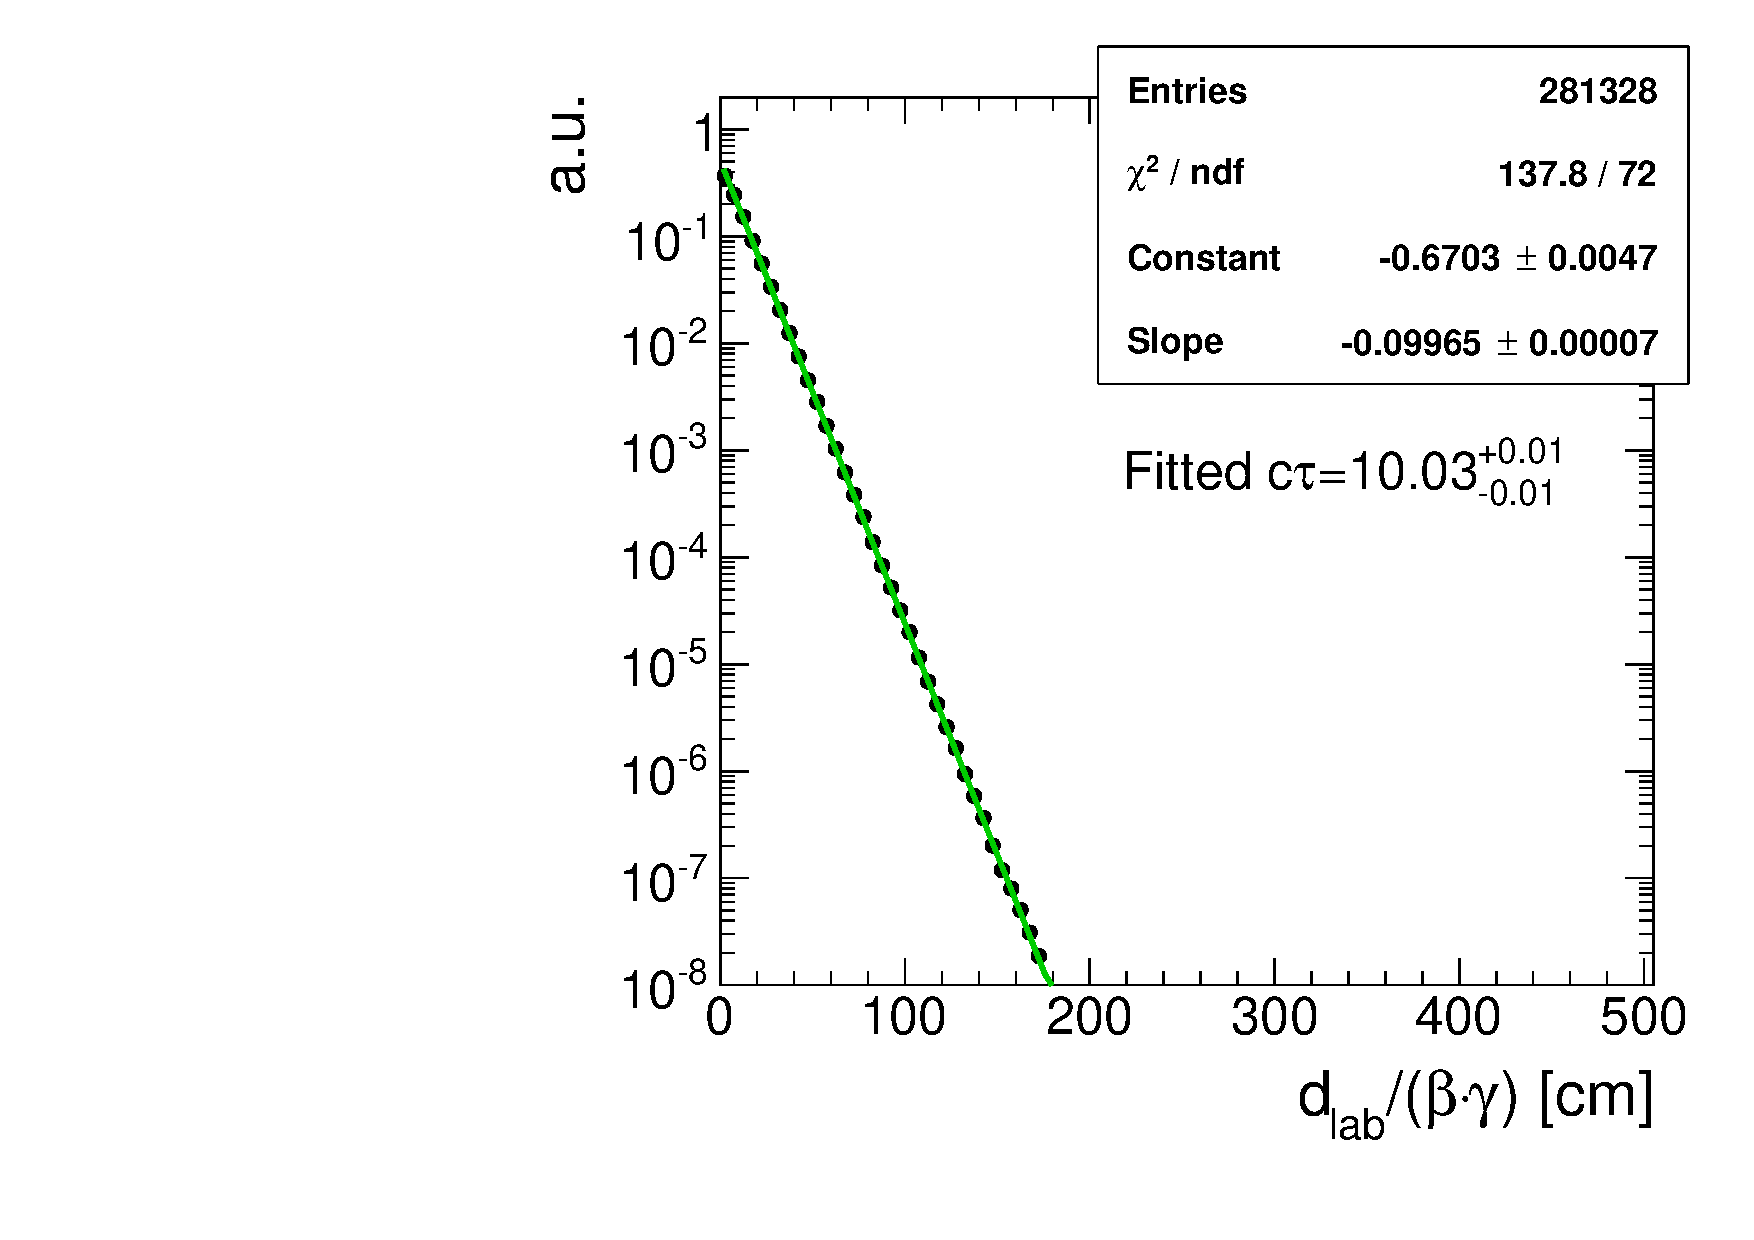
\includegraphics[width=0.49\textwidth]{figures/analysis/10cm.pdf}
  \end{tabular}
  \caption{Normalized distribution of the proper lifetime $d_{\text{lab}}/\left(\beta\gamma \right)$ of all charginos contained in a signal sample with a generated lifetime of $c\tau^{\text{gen}}=50\cm$ reweighted to a lifetime of $c\tau^{\text{target}}=10\cm$.}
  \label{fig:FeynmanDiagram}
\end{figure}


All samples were generated for different chargino masses always almost mass-degenerate to the lightest neutralino.
The mass gap between chargino and neutralino was set to 5\gev.
However, as this analysis does not make use of the other decay products and the lifetime is set in \geant, the mass gap does not play any role.
Six different masses from 100\gev to 600\gev are simulated.
This leads then to a total number of 42 signal samples.
In Table~\ref{tab:SignalCrossSections} the NLO-NLL cross sections at $\sqrt{s}=8\tev$ for $\chipm\chimp$ and $\chipm\chiO$ production 
with wino-like charginos and degeneracy between $m_{\chipm}$ and $m_{\chiO}$ are listed \cite{bib:SignalCrossSection_2012,bib:SignalCrossSection_2013}.
The cross section does not dependent on the lifetime of the chargino.
\renewcommand{\arraystretch}{1.5}
\begin{table}[!h]
\centering
\caption{Produced signal simulated samples with corresponding cross sections}
\label{tab:SignalCrossSections}
\makebox[0.99\textwidth]{
\begin{tabular}{lll}
\multicolumn{3}{c}{} \\
\toprule
 $m_{\chipm}\left[\gev\right]$ & $\sigma_{\chipm\chimp}\left[\pb\right]$  & $\sigma_{\chiO\chimp}\left[\pb\right]$ \\
\midrule
 100     &  5.8234     &  11.5132 \\
 200     &  0.37924    &  0.77661 \\
 300     &  0.06751    &  0.14176 \\
 400     &  0.01751    &  0.03758 \\
 500     &  0.00553    &  0.01205 \\
 600     &  0.00196    &  0.00431 \\
\bottomrule
\end{tabular}}
\end{table}  

%%%%%%%%%%%%%%%%%%%%%%%%%%%%%%%%%%%%%%%%%%%%%%%%%%%%%%%%%%%%%%%%%%%%%%%%%%%%%%%%%%%%%%%%%%%%%%%%%%%%%%%%%%%%%%%%%%%%%%%%%%%%%%%%%%%%%%%%%%%%%%%%%%%%%%%%%%%%%%%%%%%%%%%%%%%%%%%%%%%%
%%%%%%%%%%%%%%%%%%%%%%%%%%%%%%%%%%%%%%%%%%%%%%%%%%%%%%%%%%%%%%%%%%%%%%%%%%%%%%%%%%%%%%%%%%%%%%%%%%%%%%%%%%%%%%%%%%%%%%%%%%%%%%%%%%%%%%%%%%%%%%%%%%%%%%%%%%%%%%%%%%%%%%%%%%%%%%%%%%%%
\section{Event selection}
\label{sec:EventSelection}
\subsection{Datasets and triggers}
\begin{itemize}
\item Datasets and triggers used in the analysis
\item signal samples generated with Madgraph and pythia
\item They are decayed in Geant to only pions. Around ten different lifetimes were simulated
\item For other lifetimes: lifetime reweighting is done PLOT
\item For five diffenrent masses (100-500 GeV) 
\end{itemize}
\subsection{Preselection}
\begin{itemize}
\item Motivate different selection cuts
\item Reference DT search for most of them
\end{itemize}
\subsection{Main discriminating variables}
\begin{itemize}
\item dE/dx
\item pt
\item Show some MC signal bkg comparioson plots (only Wjets?)
\end{itemize}

%%%%%%%%%%%%%%%%%%%%%%%%%%%%%%%%%%%%%%%%%%%%%%%%%%%%%%%%%%%%%%%%%%%%%%%%%%%%%%%%%%%%%%%%%%%%%%%%%%%%%%%%%%%%%%%%%%%%%%%%%%%%%%%%%%%%%%%%%%%%%%%%%%%%%%%%%%%%%%%%%%%%%%%%%%%%%%%%%%%%
\section{Sources of backgrounds}
\label{sec:SourcesOfBackgrounds}
\begin{itemize}
\item Background consist of particles which make high energy deposits and are high pt
\item In general: Low background search
\end{itemize}
\subsection{Fake tracks}
\begin{itemize}
\item Definition of fake tracks
\item How can they fake the signal
\end{itemize}
\subsection{Muons}
\begin{itemize}
\item How can muons fake the signal
\end{itemize}
\subsection{Pions}
\begin{itemize}
\item How can pions fake the signal
\end{itemize}
\subsection{Electrons}
\begin{itemize}
\item How can electrons fake the signal
\end{itemize}
%%%%%%%%%%%%%%%%%%%%%%%%%%%%%%%%%%%%%%%%%%%%%%%%%%%%%%%%%%%%%%%%%%%%%%%%%%%%%%%%%%%%%%%%%%%%%%%%%%%%%%%%%%%%%%%%%%%%%%%%%%%%%%%%%%%%%%%%%%%%%%%%%%%%%%%%%%%%%%%%%%%%%%%%%%%%%%%%%%%%
%%%%%%%%%%%%%%%%%%%%%%%%%%%%%%%%%%%%%%%%%%%%%%%%%%%%%%%%%%%%%%%%%%%%%%%%%%%%%%%%%%%%%%%%%%%%%%%%%%%%%%%%%%%%%%%%%%%%%%%%%%%%%%%%%%%%%%%%%%%%%%%%%%%%%%%%%%%%%%%%%%%%%%%%%%%%%%%%%%%%
\section{Background estimation methods}
\label{sec:BackgroundEstimation}
\subsection{Fake background}
\subsection{Leptonic background}
\subsection{Systematic uncertainties}

%%%%%%%%%%%%%%%%%%%%%%%%%%%%%%%%%%%%%%%%%%%%%%%%%%%%%%%%%%%%%%%%%%%%%%%%%%%%%%%%%%%%%%%%%%%%%%%%%%%%%%%%%%%%%%%%%%%%%%%%%%%%%%%%%%%%%%%%%%%%%%%%%%%%%%%%%%%%%%%%%%%%%%%%%%%%%%%%%%%%
\section{Optimization of search sensitivity}
\label{sec:Optimization}
\begin{itemize}
\item Show plots
\item show table
\item Include NlostOuter here, too
\end{itemize}

%%%%%%%%%%%%%%%%%%%%%%%%%%%%%%%%%%%%%%%%%%%%%%%%%%%%%%%%%%%%%%%%%%%%%%%%%%%%%%%%%%%%%%%%%%%%%%%%%%%%%%%%%%%%%%%%%%%%%%%%%%%%%%%%%%%%%%%%%%%%%%%%%%%%%%%%%%%%%%%%%%%%%%%%%%%%%%%%%%%%
\section{Statistical Methods/ Limit setting}
\label{sec:LimitSetting}

%%%%%%%%%%%%%%%%%%%%%%%%%%%%%%%%%%%%%%%%%%%%%%%%%%%%%%%%%%%%%%%%%%%%%%%%%%%%%%%%%%%%%%%%%%%%%%%%%%%%%%%%%%%%%%%%%%%%%%%%%%%%%%%%%%%%%%%%%%%%%%%%%%%%%%%%%%%%%%%%%%%%%%%%%%%%%%%%%%%%
\section{Results}
\label{sec:Results}
\begin{itemize}
\item Data cutflowtable
\item Tables with results
\item One plot (4 bins: Prediction and data)
\end{itemize}

%%%%%%%%%%%%%%%%%%%%%%%%%%%%%%%%%%%%%%%%%%%%%%%%%%%%%%%%%%%%%%%%%%%%%%%%%%%%%%%%%%%%%%%%%%%%%%%%%%%%%%%%%%%%%%%%%%%%%%%%%%%%%%%%%%%%%%%%%%%%%%%%%%%%%%%%%%%%%%%%%%%%%%%%%%%%%%%%%%%%
\section{Interpretation}
\label{sec:Interpretation}
\subsection{Systematic uncertainties of simulated signal samples}
\subsection{Exclusion limits}
\begin{itemize}
\item 1-d limits
\item 2-d limits
\end{itemize}

